\documentclass[conference]{IEEEtran}
\IEEEoverridecommandlockouts
% The preceding line is only needed to identify funding in the first footnote. If that is unneeded, please comment it out.
\usepackage{cite}
\usepackage{amsmath,amssymb,amsfonts}
\usepackage{algorithmic}
\usepackage{graphicx}
\usepackage{textcomp}
\usepackage{xcolor}
\usepackage{url}
\usepackage{listings}
\usepackage{caption}

\captionsetup[lstlisting]{position=bottom}
\def\BibTeX{{\rm B\kern-.05em{\sc i\kern-.025em b}\kern-.08em
    T\kern-.1667em\lower.7ex\hbox{E}\kern-.125emX}}

% Suppress overfull/underfull \hbox warnings
\hfuzz=10pt        % allows overfull hboxes up to 10pt without warning
\hbadness=10000    % suppresses underfull hbox warnings
\vbadness=10000    % suppresses underfull vbox warnings


\begin{document}

\title{Serverless Dataflows}
% {\footnotesize \textsuperscript{*}Note: Sub-titles are not captured in Xplore and
%should not be used}
%\thanks{Identify applicable funding agency here. If none, delete this.}

\author{\IEEEauthorblockN{1\textsuperscript{st} Diogo Jesus}
\IEEEauthorblockA{\textit{dept. name of organisation (of Aff.)} \\
\textit{Instituto Superior Tecnico (IST), INESC-ID Lisboa}\\
Lisbon, Portugal \\
diogofjesus@inesc-id.pt}
\and
\IEEEauthorblockN{2\textsuperscript{nd} Luís Veiga}
\IEEEauthorblockA{\textit{dept. name of organisation (of Aff.)} \\
\textit{Instituto Superior Tecnico (IST), INESC-ID Lisboa}\\
Lisbon, Portugal \\
luis.veiga@inesc-id.pt}}
\maketitle

\begin{abstract}
Serverless computing has become a suitable cloud paradigm for many applications, prized for its operational ease, automatic scalability, and fine-grained pay-per-use pricing model. However, executing workflows--compositions of multiple tasks--in Function-as-a-Service (FaaS) environments remains inefficient. This inefficiency stems from the stateless nature of functions, and a heavy reliance on external services for intermediate data transfers and inter-function communication.

In this document, we introduce a decentralized DAG engine that leverages historical metadata to plan and influence task scheduling. Our solution encompasses metadata management, static workflow planning, and a worker-level scheduling strategy designed to drive workflow execution with minimal synchronization. We compare our system against WUKONG, another decentralized serverless DAG engine, and Dask Distributed, a more traditional cluster-based DAG engine. Our evaluation demonstrates that utilizing historical information significantly improves performance and reduces resource utilization for workflows running on serverless platforms.
\end{abstract}

\begin{IEEEkeywords}
Cloud Computing, Serverless, FaaS, Serverless Workflows, DAG, Metadata, Workflow Prediction
\end{IEEEkeywords}

\section{Introduction}

Serverless computing, with its Function-as-a-Service (FaaS) model, offers operational simplicity, automatic scalability, and a fine-grained pay-per-use pricing model by abstracting infrastructure management. This has led to its widespread adoption for event-driven systems, microservices, and web services on platforms like AWS Lambda\footnote{https://aws.amazon.com/pt/lambda/}, Azure Functions\footnote{https://azure.microsoft.com/en-us/products/functions}, and Google Cloud Functions\footnote{https://cloud.google.com/functions}.

This paradigm is also increasingly used to execute complex scientific and data processing workflows, such as the Cybershake~\cite{cybershake_workflow} seismic hazard analysis or Montage~\cite{montage_astronomy}, an astronomy image mosaicking workflow. These applications are structured as workflows—formally represented as Directed Acyclic Graphs (DAGs) of interdependent tasks. However, efficiently executing these complex workflows on serverless platforms remains a significant challenge. The stateless nature of serverless functions hinders direct communication, forcing data exchange between these tasks through external storage and leading to performance degradation and increased latency for data-intensive workflows.

Existing solutions, including commercial stateful functions and research prototypes like WUKONG~\cite{wukong_2}, address these issues with improved orchestration and decentralized scheduling. Yet, these approaches often rely on one-step scheduling, making decisions based solely on the immediate workflow stage without considering global implications.

In this paper, we argue that leveraging historical metadata from previous workflow runs can provide critical insights into task behavior. We propose a scheduler that uses this information to make smarter scheduling decisions, aiming to reduce overall workflow makespan and increase resource efficiency on serverless platforms.

%TODO: Contributions of our work

\section{Related Work}
\label{s:related_work}

Our work builds upon and differs from existing research in serverless workflow orchestration, which can be broadly categorised into \textbf{cloud-native stateful services}, \textbf{FaaS runtime extensions}, and \textbf{decentralized serverless schedulers}.

\subsection{Cloud-Native Stateful Orchestration}
Commercial platforms like AWS Step Functions~\cite{aws_step_functions}, Azure Durable Functions~\cite{azure_durable_functions}, and Google Cloud Workflows~\cite{google_cloud_workflows} provide a managed solution for composing serverless functions into workflows. They handle state persistence and fault tolerance, abstracting orchestration complexity from the developer. However, they are often tightly coupled with their provider's ecosystem, can introduce vendor lock-in, and are generally designed for reliability and ease of use rather than performance, optimal resource usage or data locality.

\subsection{FaaS Runtime Extensions for Data Locality}
A body of work seeks to address the fundamental data exchange inefficiency in serverless platforms through runtime modifications. \textbf{Palette}~\cite{palette_load_balancing} introduces locality ``hints'' to co-locate related function invocations on the same worker. \textbf{Faa\$T}~\cite{faast_caching} provides a transparent, auto-scaling distributed cache for serverless functions. \textbf{Lambdata}~\cite{lambdata_intents} requires developers to declare data intents (input/output objects) to enable data-aware scheduling. These solutions demonstrate the significant performance gains possible by improving data locality, but often require modifications to the application code or the underlying FaaS platform itself, limiting their portability and adoption.

\subsection{Decentralized Serverless Schedulers}
Several frameworks have been designed to execute workflows efficiently on unmodified serverless infrastructure. \textbf{PyWren}~\cite{pywren} is an early orchestrator for embarrassingly parallel computations, but its simple design can be inefficient for more complex workflows. \textbf{Unum}~\cite{unum_decentralized_orchestrator} decentralizes orchestration logic by embedding it within application code, allowing portability across different cloud providers, but offering limited data locality optimizations.

The most directly comparable work to ours is \textbf{WUKONG}~\cite{wukong_2}, a decentralized DAG engine that uses static scheduling and runtime optimizations to minimize data movement. WUKONGs' key innovations include:
\begin{itemize}
    \item \textbf{Decentralized Scheduling:} Eliminating the central scheduler bottleneck;
    \item \textbf{Task Clustering:} Forcing the execution of sequences of tasks on the same worker to reuse intermediate results and avoid using external storage;
    \item \textbf{Delayed I/O:} Heuristically postponing data writes to external storage in the hope that dependent tasks can be executed locally.
\end{itemize}

While WUKONG represents a significant advance, its scheduling and optimizations are based solely on the structure of the \textit{current} workflow DAG. It employs a \textbf{one-step scheduling} policy, making decisions using immediate runtime information without leveraging knowledge it has about the entire workflow. Besides that, WUKONG also uses optimizations based on heuristics, which can lead to suboptimal performance when workflow behavior deviates from expected patterns.

\subsection{Discussion}
The Function-as-a-Service (FaaS) model offers a transformative approach to cloud computing by abstracting infrastructure management and enabling developers to focus on business logic. Despite current platform limitations, Serverless architectures have been widely adopted for event-driven applications, microservices, IoT processing, and web services.

While researching, we explored some modern cloud-native solutions that seamlessly integrate with cloud environments. We also found innovative extensions to the FaaS runtime that aim to improve \textbf{data locality}, a technique that can enhance performance and resource efficiency of serverless workflows by reducing data transfer overheads and removing the need to use external services for synchronization.

Finally, we compared serverless workflow execution orchestrators and schedulers, from which we found WUKONG to be the most interesting, innovative and promising approach for exploiting the most out of the serverless computing paradigm. WUKONG achieves \textbf{fast scale-out times} by delegating part of the worker instancing to an external component, \textbf{scalability} with its distributed scheduling approach, and \textbf{data locality} with its optimizations that try to run related tasks on the same worker, minimizing data transfers. Despite its advantages, we also found that WUKONGs' heuristic optimizations could become inefficient in some scenarios. We believe that WUKONG scheduling decisions are optimized for workflows with short and uniform tasks.

By analyzing related works, we didn't find solutions that tried to make scheduling decisions based on the entire workflow nor that used historical information to make scheduling decisions. We saw this as a research opportunity and decided to explore it with the goal of reducing makespan of workflows running on top of FaaS while also using fewer resources, thereby improving cost efficiency and enabling a wider variety of workflows to run on top of FaaS.

\section{Architecture}
\label{s:architecture}

While current serverless platforms excel at embarrassingly parallel jobs with short-duration tasks, they present challenges for workflows involving significant data exchange between tasks due to their architectural limitations, which deny inter-function communication and control over where each function is executed. In the future, however, serverless platforms are expected to improve, eventually overcoming these limitations and becoming a viable, user-friendly and cost-effective alternative to IaaS for a wide range of workflows.

As we have stated, most existing serverless schedulers employ an approach where decisions are made based solely on the immediate workflow stage without considering the global implications. We hereby propose a novel \textit{decentralized serverless workflow execution engine} that leverages historical metadata from previous workflow runs to make fast predictions and create workflow plans before they execute. Such plans include information about where to execute each task (locality), the worker resource configuration to use (how much vCPUs and Memory) and optimizations. At run-time, the workers will execute the plan and apply the specified optimizations. It was written in \textit{Python}, a language known for its simplicity and popularity among data scientists.

\subsection{Architecture Overview}

The architecture of this decentralized serverless workflow execution engine comprises three high-level components, each with different responsibilities:

\begin{enumerate}
    \item \textbf{Metadata Management}: Responsible for collecting and storing task metadata from previous executions. It also uses this metadata to provide predictions regarding task execution times, data transfer times, task output sizes, and worker startup times;
    \item \textbf{Static Workflow Planner}: Receives the entire workflow, represented as a Directed Acyclic Graph (DAG), and a "planner" (an algorithm chosen by the user). This planner will use the predictions provided by Metadata Management to create a static plan/schedule to be followed by the workers;
    \item \textbf{Scheduler}: This component is integrated into the workers, and it is responsible for executing the plan generated by the Static Workflow Planner, applying optimizations and delegating tasks as needed.
\end{enumerate}

\subsection{Distributed Architecture}

There are three distinct computational entities in our distributed decentralized architecture:

\begin{itemize}
    \item \textbf{User Computer}: Responsible for creating workflow plans, submitting them (triggering workflow execution), and receiving its results. The planning phase also happens on this computer, right before a workflow is submitted for execution;
    \item \textbf{Workers}: These are the FaaS workers (often running in containerized environments), that execute one or more tasks. The decentralization of our solution is due to the fact that these workers are responsible for scheduling of subsequent tasks, delegating tasks and launching new workers when needed without requiring a central scheduler. Lastly, they are also responsible for collecting and uploading metadata;
    \item \textbf{Storage}: Consists of an \textit{Intermediate Storage} for intermediate outputs which may be needed for subsequent tasks and a \textit{Metadata Store} for information crucial to workflow execution (e.g., notifications about task readiness and completion).
\end{itemize}

\subsubsection{Metadata Management}
The \textbf{Metadata Management} component is central to providing accurate task-wise predictions for execution time, input/output ratio, and data transfer times. This is achieved by collecting historical data from previous workflow runs. The gathered information is stored in WUKONGs' Metadata Store, with proposed structures for task metadata and data transfer metadata.

The \texttt{task\_metadata} structure includes:
\begin{figure}[h]
\centering
\begin{lstlisting}[basicstyle=\ttfamily\footnotesize, columns=fullflexible, breaklines=true]
{
  task_id: string,
  worker_configuration: { v_cpu: number, ram: number },
  execution_time: number,
  input_size: number,
  output_size: number
}
\end{lstlisting}
\caption{Task metadata structure}
\label{lst:task_metadata}
\end{figure}

This captures details about the task's identity, the worker configuration it ran on, its execution duration, and the sizes of its inputs and outputs.

The \texttt{data\_transfer\_metadata} structure includes:
\begin{figure}[h]
\centering
\begin{lstlisting}[basicstyle=\ttfamily\footnotesize, columns=fullflexible, breaklines=true]
{
  data_size: number,
  transfer_time: number
}
\end{lstlisting}
\caption{Data transfer metadata structure}
\label{lst:data_transfer_metadata}
\end{figure}

This records the size of the data transferred and the time taken for that transfer [133, Figure 7].

This metadata is uploaded by workers after each task execution and data transfer [9]. An API, \texttt{MetadataAccess}, exposes this stored information to the Static Workflow Planner [15]. The interface for this API includes:
\begin{figure}[h]
\centering
\begin{lstlisting}[language=Java, basicstyle=\ttfamily\footnotesize, columns=fullflexible, breaklines=true]
interface MetadataAccess {
  predict_remote_download_time(data_size: number, sla?: median | percentile_value | avg): number;
  predict_output_size(task_id: string, input_size: number, sla?: median | percentile_value | avg): number;
  predict_execution_time(task_id: string, input_size: number, worker_configs: List <{ worker_config: { v_cpu: number, ram: number } }>, sla?: median | percentile_value | avg): List <{ worker_config: { v_cpu: number, ram: number }, time: number }>;
}
\end{lstlisting}
\caption{MetadataAccess interface}
\label{lst:metadata_access}
\end{figure}

These functions allow algorithms to predict download times, task output sizes, and task execution times across various worker configurations, with an optional \texttt{sla} (service-level agreement) argument to specify the desired statistical metric (e.g., median, percentile, average) for prediction guidance [16]. While research like Jolteon focuses on highly accurate, guaranteed predictions for service providers, this solution's predictions are intended to provide insights into previous executions rather than strong guarantees [17, 18].

\subsubsection{Static Workflow Planner}
The \textbf{Static Workflow Planner} module receives the workflow DAG and a user-provided algorithm, granting it access to the DAG and the \texttt{MetadataAccess} API [18]. The algorithm then produces an \textbf{Annotated DAG}, where each task's structure is extended with a \texttt{worker\_id} and specific optimization instructions [18].

The \texttt{AnnotatedTask} structure is defined as:
\begin{figure}[h]
\centering
\begin{lstlisting}[basicstyle=\ttfamily\footnotesize, columns=fullflexible, breaklines=true]
{
  task_id: string,
  worker_id: number, // worker that will execute this task
  optimizations: {
    // indicates if the worker of this task can start download data dependencies for future tasks while executing this task
    pre_load: bool,
    // the workers should the worker of this task pre_warm if appropriate (at runtime) (only makes sense for algorithms that use non_uniform workers)
    pre_warm: List <worker_ids>,
    // indicates if this task be executed more than once if needed
    task_dup: bool,
  },
  // ... other task properties
}
\end{lstlisting}
\caption{AnnotatedTask structure}
\label{lst:annotated_task}
\end{figure}

The \texttt{worker\_id} designates the worker instance for the task, similar to "colors" in Palette, to improve data locality [6, 19, 20]. Optimizations include \texttt{pre\_load} (allowing data dependencies for future tasks to be downloaded concurrently with current task execution), \texttt{pre\_warm} (pre-invoking workers to reduce cold starts, particularly relevant for non-uniform workers), and \texttt{task\_dup} (allowing a task to be executed more than once if beneficial, e.g., to avoid waiting for data) [20, 21].

Users can select from a range of algorithms or implement their own by adhering to the \texttt{PlanningAlgorithm} interface [22]:
\begin{figure}[h]
\centering
\begin{lstlisting}[language=Java, basicstyle=\ttfamily\footnotesize, columns=fullflexible, breaklines=true]
interface PlanningAlgorithm {
  plan(dag: OriginalDAG, metadataAccess: MetadataAccess, sla: median | percentile_value | avg): Tuple <AnnotatedDAG, WorkerConfigurationMapping>
}
\end{lstlisting}
\caption{PlanningAlgorithm interface}
\label{lst:planning_algorithm}
\end{figure}
The algorithm must also output a \texttt{WorkerConfigurationMapping}, which maps \texttt{Worker IDs} to their respective \texttt{Worker Configurations} (vCPU and RAM) [23]:
\begin{figure}[h]
\centering
\begin{lstlisting}[basicstyle=\ttfamily\footnotesize, columns=fullflexible, breaklines=true]
Map <
  worker_id: number,
  worker_configuration: { v_cpu: number, ram: number }
>
\end{lstlisting}
\caption{WorkerConfigurationMapping structure}
\label{lst:worker_configuration_mapping}
\end{figure}
Two algorithms are proposed for implementation [23, 24]:
\begin{enumerate}
    \item A **uniform Lambda worker algorithm**: This algorithm uses the \texttt{MetadataAccess} API to predict and optimize the longest workflow path (critical path) by simulating the \texttt{pre-load} optimization. It iteratively optimizes the critical path until no further improvements can be made, providing a benchmark against WUKONG 2.0 to assess the value of historical metadata [23, 24].
    \item A **non-uniform worker algorithm**: This algorithm first identifies the critical path assuming all tasks run on the most performant worker configuration. It then strategically downgrades resources on other paths to maximize resource efficiency without creating new critical paths. After tasks are attributed to workers at plan-time, it simulates additional optimizations to further enhance resource efficiency and reduce makespan [24]. This algorithm aims for better performance and resource efficiency by masking data transfer latency and minimizing large data transfers [24].
\end{enumerate}
Future enhancements could include defining "re-planning points" within the workflow, allowing the initial plan to be dynamically adjusted during runtime based on updated metadata for greater precision, though this introduces potential overhead [25].

\subsubsection{Scheduler}
The \textbf{Scheduler} component is integrated into the workers and is responsible for executing the plan generated by the Static Workflow Planner [25]. By having foreknowledge of task placements, the Scheduler can apply various optimizations defined by the algorithm [25]. These optimizations include [21]:
\begin{itemize}
    \item \textbf{Pre-warm}: Sending empty invocations to FaaS workers to reduce cold start latencies and achieve a shorter workflow makespan [21].
    \item \textbf{Pre-load}: Allowing a worker, designated to execute a downstream task, to begin downloading its data dependencies from remote storage concurrently while it executes other tasks. This parallelizes data download and can reduce overall makespan [21].
    \item \textbf{Task-dup} (Task duplication): If a worker is waiting for data from an upstream task (currently executing or pending on another worker), it can execute that upstream task itself. This can reduce makespan and save data download time, as the waiting worker no longer needs to wait for the data to be uploaded to external storage and then download it [21].
\end{itemize}

To illustrate the impact of these scheduling approaches, consider a workflow with Task 1 outputting large data, and Task 2 also feeding into Task 5, which also depends on Task 1.

In \textbf{WUKONGs' approach}, if Task 1's output is large, its worker attempts to execute all downstream tasks (e.g., Task 3, Task 4, and Task 5) locally to avoid large data transfers [26]. Assuming Task 2 finishes after Task 1, Task 1's worker would execute Tasks 3 and 4, then check if Task 5 is ready. If Task 2 hasn't finished, Task 1's worker begins uploading its large output to external storage. Task 5 would only run after this upload, and potentially a download by another worker [26]. This can be inefficient if Task 2 then finishes, but Task 5's worker still has to wait for Task 1's output, which was unnecessarily delayed [26].

With a \textbf{plan-based approach}, as soon as Task 1's worker finishes, it immediately uploads Task 1's output to external storage, knowing it will not execute Task 5 [27]. This means when Task 5 is ready to execute (i.e., Task 2 is complete), it only needs to download Task 1's output, as the upload has already occurred, potentially in parallel with other computations [27]. This is effective because the worker knows its exact role from the plan [27].

By adding \textbf{optimizations like pre-warming and pre-loading}, the plan-based approach can be further enhanced [28]. For example, Task 1's worker can pre-warm the worker designated for Task 3, reducing cold start latency [28]. Simultaneously, if Worker 2 needs Task 1's output for Task 5, it can start downloading Task 1's output while it executes Task 2 [28]. This pre-loading of data dependencies in parallel significantly helps in reducing the overall workflow makespan [28].

\subsection{Workflow Definition Language}

The user can create workflows by composing individual Python functions, as shown in listing \ref{lst:dag_lang_example}. Here, we define two tasks, \texttt{task\_a} and \texttt{task\_b}, and then compose them into a DAG/Workflow by passing their results as arguments to the next task. The resulting workflow can be visualized in figure \ref{fig:dag_example}.

\begin{figure}[h]
\centering
\begin{lstlisting}[language=Python, basicstyle=\ttfamily\footnotesize, columns=fullflexible, breaklines=true]
# 1) Task definition
@DAGTask
def task_a(a: int) -> int:
    # ... user code logic ...
    return a + 1

@DAGTask
def task_b(*args: int) -> int:
    # ... user code logic ...
    return sum(args)

# 2) Task composition (DAG/Workflow)
a1 = task_a(10)
a2 = task_a(a1)
a3 = task_a(a1)
b1 = task_b(a2, a3)
a4 = task_a(b1)
\end{lstlisting}
\caption{DAG definition example}
\label{lst:dag_lang_example}
\end{figure}

\begin{figure}[h]
    \centering
    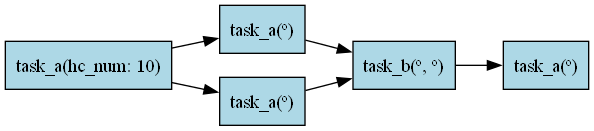
\includegraphics[width=\columnwidth]{figures/dag_lang_example.png}
    \caption{Simple DAG example}
    \label{fig:dag_example}
\end{figure}

When \texttt{task\_a(10)} is invoked, it doesn't actually run the user code. It instead creates a representation of the task, which can be passed as argument to other tasks. The workflow planning and execution only happens once \texttt{.compute()} is called on the last/sink task (\texttt{a4}), as shown in listing \ref{lst:triggering_workflow_execution}. When \texttt{compute()} is called, we can create a representation of the entire workflow structure by backtracking the task dependencies.

\begin{figure}[h]
\centering
\begin{lstlisting}[language=Python, basicstyle=\ttfamily\footnotesize, columns=fullflexible, breaklines=true]
result = a4.compute(
    dag_name="simpledag", 
    config=Worker.Config(
        faas_gateway_address=...,
        intermediate_storage_config=(ip, port, password),
        metrics_storage_config=(ip, port, password),
        planner_config=SimplePlannerAlgorithm.Config(
            sla=sla,
            worker_resource_configuration=TaskWorkerResourceConfiguration(cpus=3, memory_mb=512),
        )
    )
)
\end{lstlisting}
\caption{Triggering workflow execution}
\label{lst:triggering_workflow_execution}
\end{figure}

It's important to note that this DAG definition language doesn't support "dynamic fan-outs" (e.g., creating a variable number of tasks depending on the result of another task).

% ------------------------------------------------ %

\section{Evaluation and Analysis}

\subsection{Testing Environment}
%TODO: explain Docker simulating faas environment
\subsection{Testing Configurations}
%TODO: worker resources, workflows, planners, SLAs

\section{Conclusion}

\bibliographystyle{IEEEtran}
\bibliography{references}

\end{document}
